\newcommand{\gol}{\emph{GameOfLife}}

\section{Opgave 3}

\subsection{Specifikation}
Der ønskes et program, der kan udfører simuleringer af celle liv efter modellen \emph{Conway's Game of Life},
se evt \url{http://en.wikipedia.org/wiki/Game_of_life}.

følgende er implimenteret:
\begin{itemize}
  \item et \emph{GameOfLife} objekt, der dog også kan håndterer andre cellulare automier.
  \item Constructor der tillader at initalisere et \emph{GameOfLife} objekt
  med en given størrelse, tilfældigt eller ej.
  \item Constructor der tillader at initalisere et \emph{GameOfLife} objekt
  med en given start tilstand.
  \item Mulighed for at tage et enkelt skridt frem.
  \item Mulighed for at tage skridt kontinuert.
  \item Mulighed for at hente \emph{GameOfLife} objekter fra filer.
  \item Mulighed for at hente andre regelsæt end game of life fra filer.
  \item Mulighed for at hente farve fra filer.
  \item Mulighed for at manipulerer \emph{GameOfLife} objekter med musen.
  \item ``Banen'' er sat op som en torus, dvs. kanterne rører hinanden.
\end{itemize}

\subsection{Design}

\subsubsection{ GameOfLifeMain klassen }
Dette er en statisk klasse, der lader en bruger lege med \emph{GameOfLife} klassen.
Brugeren kan lave og manipulerer et \emph{GameOfLife} objekt her.

Et dummy \emph{GameOfLife} objekt tegnes på et $512\times512$ canvas og
brugeren bedes om at vælge mellem at hente et sæt filer, lave en tilfældig bane eller en ``ren'' bane.

Brugeren kan nu simulerer enkelte skridt ved at trykke på \emph{mellemrum},
eller flere ved at holde tasten.

Brugeren kan også manipulerer celler med musen.

\paragraph{ GameOfLife  initialsering }
Brugeren bedes om at vælge mellem 3. muligheder.

Skrives ordet \emph{random}, spørges om en størrelse og et \gol~objekt laves med denne størrelse, tilfældig farve og starttilstand.

Skrives ordet \emph{clean}, spørges om en størrelse og et \gol~objekt laves med denne størrelse, tilfældig farve og alle celler som døde.

Skrives ordet \emph{load}, spørges om en sæt filer.
Regelfil, starttilstandsfil og farvefil. Både regel- og farvefilen accepterer ``N'';
I hvilket tilfælde Conway's Game of Life hhv. tilfældige farver benyttes.

\paragraph{ Skridt }
Der tages et skridt, hver gang der trykkes på mellemrum. Holdes denne inde skriver maskinen naturligvis flere til key-bufferen.
Denne tømmes, hvert skridt - da hvert skrict kan tage lang tid at udregne og simulieringen ikke ville stoppe, når mellemrumstasten løftes da.

Skærmen gentegnes IKKE hvid mellem hvert skridt, dette medvirker at alias-fejl undertrykkes.

\paragraph{ Mussemanipulation }
Trykkes der med musen, gemmes værdien af cellen under den. Så længe den holdes, sættes celler under den til denne værdi plus én.
\gol~objektet holder styr på at ``folde'' værdier, så en levende celle bliver til en død, i stedet for en celle uden regler.


\subsubsection{ GameOfLife klassen}

\gol~klassen har følgende data:
\begin{itemize}
  \item int edgeState; Bestemmer hvilen tilstand sidderne har. -1 for en torus.
  \item int[][] state; Gemmer data om værdien i alle celler. Dette array forudsættes at være med lige kanter, og ikke tomt.
  \item int[][] rules; Gemmer regelsættet
  \item int states; Antallet af forskellige states, det samme som rækkeantallet i rules.
  \item Color[] colors; Array af farver til cellerne.
\end{itemize}




\paragraph{ GameOfLife(int, int, boolean)} Laver et \gol~objekt med Conway's regler og en given størrelse. Der kan vælges en tilfældig starttilstand.

\paragraph{ GameOfLife(int[][]) } Laver et \gol~obejkt med Conway's regler og en given starttilstand. Er denne ikke valid laves et \gol~med én celle.

\paragraph{GameOfLife()} aver et \gol~obejkt med Conway's regler og én celle.

\paragraph{setRules(int[][])} Sætter et regelsæt, hvis dette er gyldigt og ingen celler lever, der ikke findes i regelsættet.
I et regelsæt er hver række regelsættet for en celletilstand, første kolonne angiver antalet af ``liv'' denne tælder for,
mere om dette under \emph{neighbors}, de næste kolonner angiver, hvad der sker med denne celle, når summen af ``liv''
omkring den har forskellige værdier. første kolonne er ved 0 eller mindre, næste 1, så 2 osv. et større antal liv ender altid i kolonnen længst til højre.

kalder \emph{addMissingColors()}

\paragraph{setRules()} Sætter regelsættet til \emph{Conway's Game of Life}

\paragraph{addMissingColors()} Tilføjer farver til alle celletyper uden farver.

\paragraph{neighbors(int, int)} Udregner antallet af naboliv for en given celle,
dette gøres ved at kigge på cellerne rundt om og aflæse mængden af ``liv'' denne tæler for i \emph{rules}.
Dem under, dem ved siden af og dem over. 
Er \emph{edgeState}=-1 kaldes \emph{mod} på begge komposanter for koordinatet til celler rundt om,
dette gør at ex celle$(10, 5)$ med state størrelse $(10, 10)$ bliver til celle$(0, 5)$

\paragraph{step()} Udregner næste tilstand for alle celler, og sætter dem til dette.
For hver celle kaldes \emph{neighbors} og det aflæses i \emph{rules}, hvilken celle de så skal blive til

\paragraph{render(double, double, double, double)} Tegner alle celler i det specificerede område.

\paragraph{renderMouse(double, double, double, double)} Tegner en rød markør for musen, låst til cellegitteret, når cellerne tegnes i det specificerede område.

\paragraph{mouseX(double, double, double, double)} Retunerer musens X komposant i antal celler, når disse tegnes i det specificerede område.
Er musen udenfor retuneres -1.

\paragraph{mouseY(double, double, double, double)} Retunerer musens Y komposant i antal celler, når disse tegnes i det specificerede område.
Er musen udenfor retuneres -1.

\paragraph{toString()} Skriver tilstanden af alle celler til konsollen med celle(0,0) i øverste, venstre hjørne.

\paragraph{printNeighbors()} Skriver antallet af naboer for alle celler til konsollen med celle(0,0) i øverste, venstre hjørne.

\paragraph{mod(int, int)} Folder et tal om, så det ligger mellem 0 og 2. argument. ex: mod$(10, 9) = 1$, mod$(-1, 2) = 1$

\paragraph{alterState(int, int)} Ændre den givne celle, til den næste i regelsættet.

\paragraph{setState(int, int, int)} Sætter den givne celle til en værdi. Folder rundt, så en celle sat til 4, når der kun er 3 typer bliver 0.

\paragraph{setStates(int[][])} Sikker sætter for alle celler. Ændre kun celler, hvis det givne array er ``lige'' og ingen celler ikke findes i regelsættet.

\paragraph{getRules()} Retunerer en kopi af regelsættet.

\paragraph{getColors()} Retunerer en kopi af farvesættet.

\paragraph{getStates()} Retunerer antallet af regler/celletyper.

\paragraph{getState()} Retunerer en kopi af celle-stadie-arrayet.

\paragraph{getState(int, int)} Retunerer celle-typen i det givne koordinat.

\paragraph{validRules(int[][])} Checker om et givent regelsætr er validt og om der findes celler, ikke specificerert i dette.

\paragraph{setColors(Color[])} Sætter farvesættet til dette. Tilføjer manglende farver.

\paragraph{loadSetup(String, String, String, boolean)} Indhenter et fuldt setup, regler, states, farver. regler og farver kan undlades ved argument ``N''.
retunerer sand ved succes. Kan printe hvad fejlen er, hvis en opstår.

\paragraph{loadSetup(int[][], int[][], Color[], boolean)} Indhenter et fuldt setup, regler, states, farver.
retunerer sand ved succes. Kan printe hvad fejlen er, hvis en opstår.

\paragraph{loadSetup(int[][], Color[], boolean)} Samme som ovenfor, men med \gol~regler

\paragraph{loadSetup(int[][], boolean)} Samme som ovenfor, men tilfældige farver.

\paragraph{randomize()} Sætter alle celler til tilfældige værdier.

\subsection{test}

\subsubsection{\gol~ klassen}
\gol~klassen testes udelukkende fra konsollen. Klassen \emph{GameOfLifeTest} køres.
Denne laver et tilfældig $5\times5$ \gol~objekt, printer det til konsollen, printer naboer, tager et skridt og printer sig selv igen.
dette giver:
\begin{lstlisting}[caption="test af \gol~objekt"]
State:
1 I 1 0 I 
I 0 0 0 0 
0 0 0 1 0 
0 0 1 0 1 
I I 0 1 0 

Neighbors:
5 5 3 3 4 
3 4 3 3 4 
2 2 2 2 3 
3 3 3 4 3 
5 5 5 4 5 

State:
0 0 1 1 0 
1 0 1 1 0 
0 0 0 1 1 
1 1 1 0 1 
0 0 0 0 0 
\end{lstlisting}

Det ses at naboer udregnes korrekt, også rundt om kanter (cellen i øverste venstre hjørne har 5 naboer, markeret med I'er, dette er rettet manuelt).
Det ses ligeledes at de skifter til de rigtige naboer.

\subsubsection{\gol\emph{Main} klassen}

Først testes for fejlinputs:
\begin{lstlisting}[caption="test af feljinputs"]
Type "load" to load a file set,
Type "random" to initialize a random game of life,
Type "clean" to initialize a random game of life:
derp
Wrong intput
>> App lukkes og åbnes på ny

Type "load" to load a file set,
Type "random" to initialize a random game of life,
Type "clean" to initialize a random game of life:
random
width:
derp
Please enter positive values
>> App lukkes og åbnes på ny

Type "load" to load a file set,
Type "random" to initialize a random game of life,
Type "clean" to initialize a random game of life:
clean
width:
-9000
Please enter positive values
>> App lukkes og åbnes på ny

Type "load" to load a file set,
Type "random" to initialize a random game of life,
Type "clean" to initialize a random game of life:
load
Write filename for rules, N for Game of life
hurr
Write filename for initial state
durr
Write filename for colorfile, N for random
derp
Error loading file: hurr
Error in loading
\end{lstlisting}

Dernæst testes den tilfældige \gol~generereing, dette giver resultatet i figur~\ref{fig:rand}
\begin{lstlisting}[caption=" Tilf\ae ldigt game of life p\aa 50x50"]
Type "load" to load a file set,
Type "random" to initialize a random game of life,
Type "clean" to initialize a random game of life:
random
width:
50
height:
50
\end{lstlisting}

\begin{figure}
        \centering
        \begin{subfigure}[b]{0.3\textwidth}
                \centering
                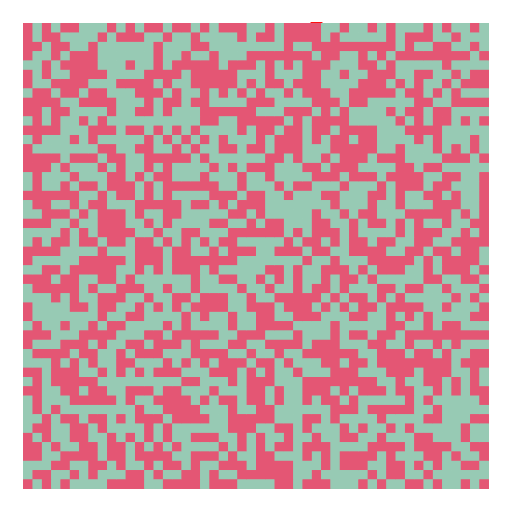
\includegraphics[width=\textwidth]{rand1.png}
                \caption{Ved start}
        \end{subfigure}%
        ~
        \begin{subfigure}[b]{0.3\textwidth}
                \centering
                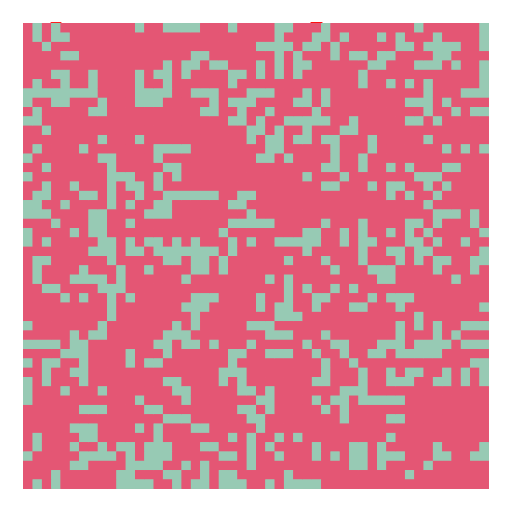
\includegraphics[width=\textwidth]{rand2.png}
                \caption{Efter 1 skridt}
        \end{subfigure}
        ~
        \begin{subfigure}[b]{0.3\textwidth}
                \centering
                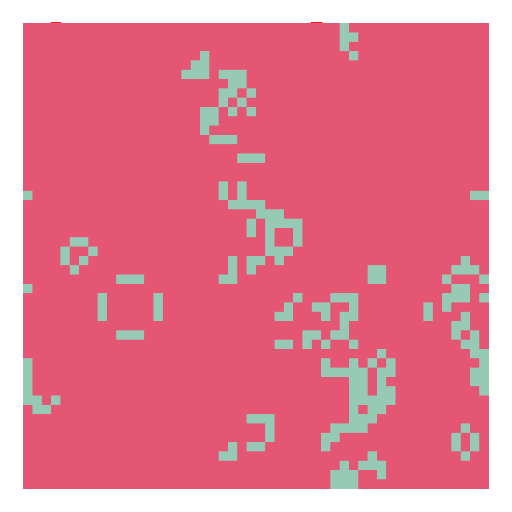
\includegraphics[width=\textwidth]{rand3.png}
                \caption{Efter mange skridt}
        \end{subfigure}
        \caption{tilfældige \gol~objekter med størrelse $50\times50$}\label{fig:rand}
\end{figure}

Dernæst testes den ``rene'' \gol~generereing, og denne manipuleres med musen. Dette giver resultatet i figur~\ref{fig:mani}
\begin{lstlisting}[caption=" Tilf\ae ldigt game of life p\aa 50x50"]
Type "load" to load a file set,
Type "random" to initialize a random game of life,
Type "clean" to initialize a random game of life:
clean
width:
25
height:
25
\end{lstlisting}

\begin{figure}
        \centering
        \begin{subfigure}[b]{0.3\textwidth}
                \centering
                
\includegraphics[width=\textwidth]{mani1.png}
                \caption{Ved start}
        \end{subfigure}%
        ~
        \begin{subfigure}[b]{0.3\textwidth}
                \centering
                
\includegraphics[width=\textwidth]{mani2.png}
                \caption{Efter manuel tilføjelse af glider}
        \end{subfigure}
        ~
        \begin{subfigure}[b]{0.3\textwidth}
                \centering
                
\includegraphics[width=\textwidth]{mani3.png}
                \caption{Efter mange skridt}
        \end{subfigure}
        \caption{``rent'' \gol~objekter med størrelse $25\times25$ manipuleret af musen}\label{fig:mani}
\end{figure}

Dernæst testes inhentning af filer. Regelsættet \emph{Brian's Brain} benyttes, se \url{http://en.wikipedia.org/wiki/Brian's_Brain};
\emph{acorn.gol} benyttes som udgangsposition, men der tilføjes lidt ekstra og farvefilen \emph{cypher.col} benyttes. Dette giver resultatet i figur~\ref{fig:file}
\begin{lstlisting}[caption=" Tilf\ae ldigt game of life p\aa 50x50"]
Type "load" to load a file set,
Type "random" to initialize a random game of life,
Type "clean" to initialize a random game of life:
load
Write filename for rules, N for Game of life
GameOfLife/briansBrain.rul
Write filename for initial state
GameOfLife/acorn.gol
Write filename for colorfile, N for random
GameOfLife/cypher.col
\end{lstlisting}
Denne bør dog ses i animation, da \emph{Brian's Brain} efter min mening er en af de smukkeste, og mest livige regelsæt.
Da alle celler dør, og celler fødes meget nemt, er næsten alt et spaceship, eller en puffer.

\begin{figure}
        \centering
        \begin{subfigure}[b]{0.3\textwidth}
                \centering
                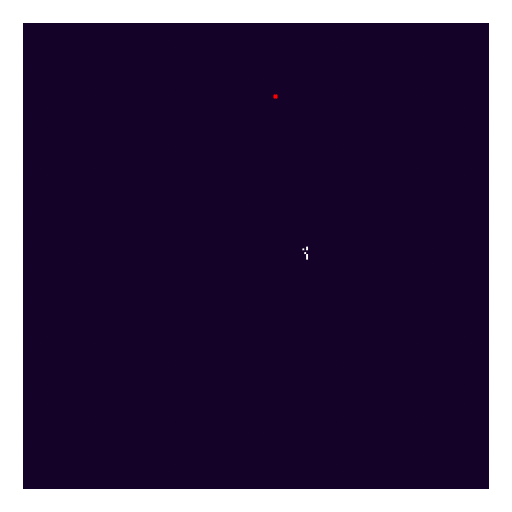
\includegraphics[width=\textwidth]{fil1.png}
                \caption{Ved start}
        \end{subfigure}%
        ~
        \begin{subfigure}[b]{0.3\textwidth}
                \centering
                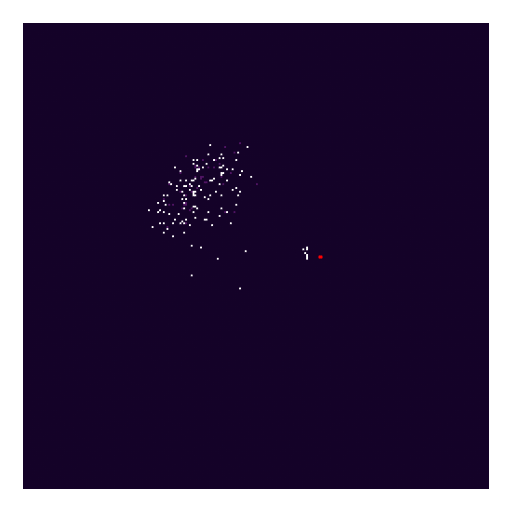
\includegraphics[width=\textwidth]{fil2.png}
                \caption{Efter tilføjelse af ``støj''}
        \end{subfigure}
        ~
        \begin{subfigure}[b]{0.3\textwidth}
                \centering
                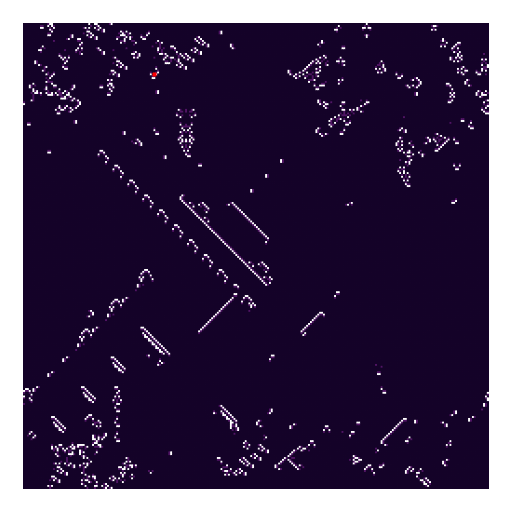
\includegraphics[width=\textwidth]{fil3.png}
                \caption{Efter mange skridt}
        \end{subfigure}
        \caption{\gol~objekter lavet fra filer}\label{fig:fil}
\end{figure}